Liczba Catalana jest to liczba ścieżek długości \(2n\) w kwadracie \(n \times n\) ,,poniżej'' przekątnej (lub na jej poziomie), idących za każdym razem jednostkę do góry lub jednostkę w prawo. Ścieżki takie nazywamy ścieżkami Dycka. Niezwykle formalna definicja. To jest jedna z tych rzeczy, które chyba po prostu trzeba narysować.

\begin{figure}[h]
	\centering
	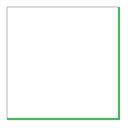
\includegraphics[scale=0.5]{images/catalan/all_paths_1.png}
  \caption{Ścieżki Dycka długości 2; \(c_1 = 1\)}
\end{figure}

\begin{figure}[h]
	\centering
	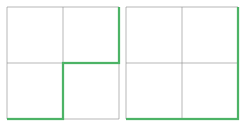
\includegraphics[scale=0.5]{images/catalan/all_paths_2.png}
  \caption{Ścieżki Dycka długości 4; \(c_2 = 2\)}
\end{figure}

\begin{figure}[ht]
	\centering
	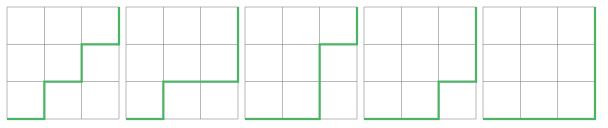
\includegraphics[scale=0.5]{images/catalan/all_paths_3.png}
  \caption{Ścieżki Dycka długości 6; \(c_3 = 5\)}
\end{figure}


\subsection{Wzór kombinatoryczny}
\begin{theorem}[Wzór kombinatoryczny na liczby Catalana]
	\begin{equation}
		c_n = \frac{1}{n+1} \cdot \binom{2n}{n}
	\end{equation}
\end{theorem}

Mamy sobie nasz kwadrat \(n \times n\). Przekątną możemy opisać tak jakby wzorem \(y = x\) (tak intuicyjnie, bo nie działamy w żadnym układzie współrzędnych, bla bla bla). Robimy sobie teraz prostą \(y = x+1\), idącą jakby ,,o jednostkę wyżej''. Zauważamy, że jeśli jakaś ścieżka przekracza linię naszej przekątnej, to musi ,,dotknąć'' linii \(y = x+1\). \textit{To widać}. Teraz wpadamy na świetny pomysł; jeśli jakaś ścieżka idąca po tym kwadracie ,,spotyka się'' z \(y = x+1\), to od tego momentu odbijamy ją symetrycznie względem \(y = x+1\). Zauważamy, że ścieżka ta (po odbiciu) skończy się w punkcie \((n-1, n+1)\) zamiast w \((n,n)\). Fakt ten dowodzimy stosując dowód przez rysowanie.

\begin{figure}[ht]
	\centering
	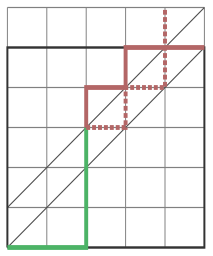
\includegraphics[scale=0.5]{images/catalan/path_with_reflection_1.png}
	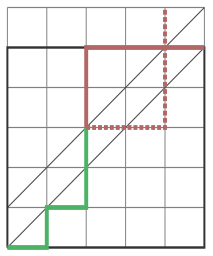
\includegraphics[scale=0.5]{images/catalan/path_with_reflection_2.png}

	\caption{Przykłady odbicia niepoprawnej ścieżki}
\end{figure}

Zauważamy fascynujący fakt, mianowicie dwie różne ścieżki będą mieć 2 różne odbicia, a więc nasze przekształcenie jest iniektywne. Ponadto, jak sobie zobaczymy jakąkolwiek ścieżkę zaczynającą się w \((0,0)\), ale kończącą się w \((n-1,n+1)\), to jesteśmy w stanie zobaczyć gdzie pierwszy raz przecina się z \(y = x+1\), a następnie ją odbić, otrzymując ścieżkę idącą do \((n,n)\) i niebędącą ścieżką Dycka, której odbicie daje wyjściową ścieżkę. Zatem odbijanie jest suriektywne. A to oznacza tylko jedną rzecz: bijekcję między ścieżkami które ,,nie są catalanowe'', a ścieżkami ,,odbitymi''.

Wszystkich możliwych ścieżek od \((0,0)\) do \((n,n)\) mamy \(\binom{2n}{n}\), bo długość naszej drogi ma \(2n\) i wybieramy sobie \(n\) miejsc gdzie idziemy w prawo. Wszystkich możliwych ścieżek od \((0,0)\) do \((n-1,n+1)\) (czyli tych które są ,,złe'') mamy \(\binom{2n}{n-1}\), bo, analogicznie, ścieżka jest długości \(2n\) ale w prawo idziemy \(n-1\) razy. To prowadzi nas do wyniku:
\begin{equation*}
	\begin{split}
		c_n
		&= \binom{2n}{n} - \binom{2n}{n-1} \\
		&= \frac{(2n)!}{n! \cdot n!} - \frac{(2n)!}{(n-1)! \cdot (n+1)!} \\
		&= \frac{(n+1) \cdot (2n)!}{n! \cdot (n+1)!} - \frac{n \cdot (2n)!}{n! \cdot (n+1)!}\\
		&= \frac{(2n)!}{n! \cdot (n+1)!} \\
		&= \frac{1}{n+1} \cdot \frac {(2n)!}{n! \cdot n!} \\
		&= \frac{1}{n+1} \cdot \binom{2n}{n}
	\end{split}
\end{equation*}
\subsection{Zależność rekurencyjna}

\begin{theorem}[Wzór rekurencyjny na liczby Catalana]
	\begin{equation}
		c_n = c_{0} \cdot c_{n-1} + c_{1} \cdot c_{n - 2} + \dots + c_{n-1} \cdot c_0
	\end{equation}
\end{theorem}

\begin{proof}
	Znowuż mamy kwadrat \(n \times n\), ale tym razem dorysowujemy sobie prostą \(y = x - 1\). Każda ścieżka przetnie kiedyś tę linię i każda ścieżka dotknie kiedyś przekątnej \(y = x\) (można to udowodnić machając i pokazując na rysunek). Rzecz teraz ma się tak, że jeśli po ,,spotkaniu się'' z \(y = x - 1\) idziesz do góry, to potem musisz odbić w prawo (lub w skrajnym przypadku skończyłeś poprawną ścieżkę). Jednocześnie pierwszy wybór kierunku (tzn. ten w punkcie \((0,0)\) zawsze jest ,,w prawo'', bo jeśli ktoś pójdzie ,,do góry'' to znajdzie się w \((0,1)\), powyżej przekątnej \(y = x\)).

	Bierzemy sobie zatem pierwsze miejsce gdzie spotkałeś się z \(y = x\) i zauważamy, że jeśli dane jest ono jakimiś współrzędnymi \((i,i)\) to przecięliśmy \(y = x-1\) w \((i,i-1)\). Ponadto, ścieżka którą szliśmy od punktu \((1,0)\) do \((i,i-1)\) tak naprawdę jest ścieżką Dycka w kwadracie od punktów \((1,0)\), \((i, i-1)\) (kwadrat ten ma długość \(i-1\)). Ależ plot twist! Ścieżka którą idziemy od punktu \((i,i)\) do \((n,n)\) jest zaś już po prostu ścieżką Dycka w kwadracie o długości boku \(n-i\). Ścieżki te są od siebie niezależne i w ogóle, a długości tych ,,kwadratów catalanowych'' sumują się do \(i - 1 + n - i = n - 1\), więc teraz możemy zmajstrować wzór (w zależności od długości boków kwadratów, które z kolei są dyktowane tym kiedy się ,,spotkamy'' z \(y = x\)):
	\begin{equation*}
		c_n = \sum_{i = 0}^{n-1} c_i \cdot c_{n-1-i}
	\end{equation*}
	Co już można odwinąć do postaci która była w twierdzeniu.

	\begin{figure}[H]
		\centering
		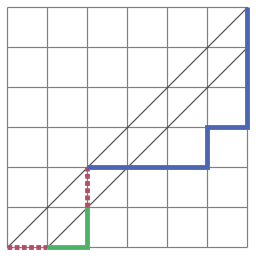
\includegraphics[scale=0.5]{images/catalan/recursive_construction_1.png}
		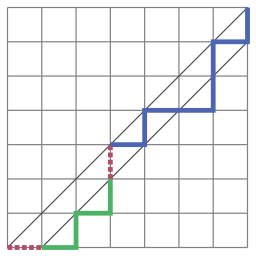
\includegraphics[scale=0.5]{images/catalan/recursive_construction_2.png}

		\caption{Przykłady ,,podzielenia'' poprawnej ścieżki Dycka na podścieżki}
	\end{figure}

\end{proof}
